\usetikzlibrary{datavisualization}
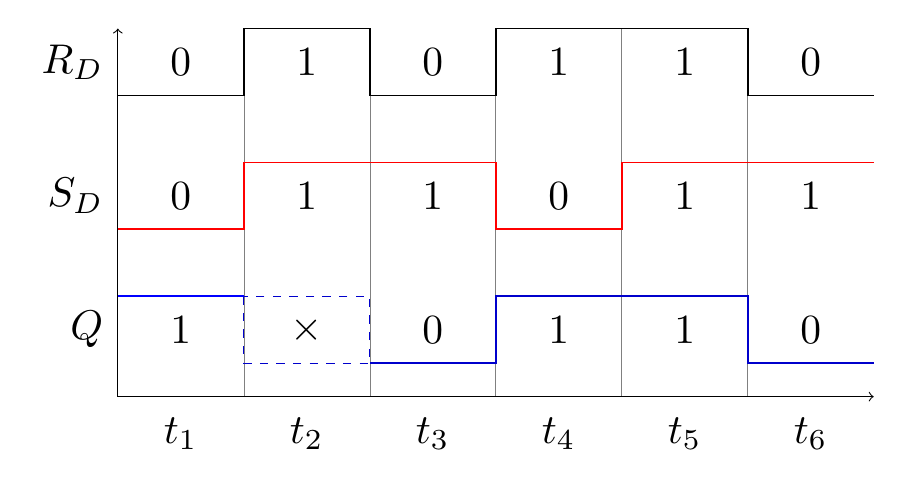
\begin{tikzpicture}[xscale=1.6, yscale=0.85]

\foreach \x in { 1,...,5 }
    \draw[help lines] (\x, 1) -- (\x, -4.5);
\foreach \x/\l in { 0.5/1,1.5/2,2.5/3,3.5/4,4.5/5,5.5/6 }
    \node[below, scale=1.5] at (\x, -4.6) {$t_{\l}$};
\foreach \x/\l in { 0.5/0,1.5/1,2.5/0,3.5/1,4.5/1,5.5/0 }
    \node[scale=1.5] at (\x, 0.5) {$\l$};
\foreach \x/\l in { 0.5/0,1.5/1,2.5/1,3.5/0,4.5/1,5.5/1 }
    \node[scale=1.5] at (\x, -1.5) {$\l$};
\foreach \x/\l in { 0.5/1,1.5/\times,2.5/0,3.5/1,4.5/1,5.5/0 }
    \node[scale=1.5] at (\x, -3.5) {$\l$};

\draw[->] (0,-4.5) -- (6,-4.5);
\draw[->] (0,-4.5) -- (0,1);

\draw[dashed,blue!80!black] (1, -3) rectangle (2, -4);


\datavisualization [
  xy Cartesian,
  visualize as line/.list={R,S,O,O2},
  S={style={red}},
  O={style={blue}},
  O2={style={blue!80!black}},
]
  data[set=R] {
    x, y
    0, 0
    1, 0
    1, 1
    2, 1
    2, 0
    3, 0
    3, 1
    5, 1
    5, 0
    6, 0
  }
  data[set=S] {
    x, y
    0, -2
    1, -2
    1, -1
    3, -1
    3, -2
    4, -2
    4, -1
    6, -1
  }
  data[set=O] {
    x, y
    0, -3
    1, -3
  }
  data[set=O2] {
    x, y
    2, -4
    3, -4
    3, -3
    5, -3
    5, -4
    6, -4
  }
  ;

  \node[left, scale=1.5] at (0,  0.5){$R_D$};
  \node[left, scale=1.5] at (0, -1.5){$S_D$};
  \node[left, scale=1.5] at (0, -3.5){$Q$};
\end{tikzpicture}